\chapter{Implementation}
  \section{Deep Learning Framework}
    TensorFlow \cite{tensorflow} was chosen as the deep learning framework for this
    project. Many others such as Caffe, Neon, Theano, and Torch are popular\cite{Bahrampour2016}.
    The main advantages of tensorflow are flexibility with running code on diverse
    hardware platforms and good support for visualisations
    of computation graphs. The other frameworks infact are more efficient
    \footnote{TensorFlow even came last in one benchmark performed on the VGG-16 network, \url{https://github.com/aizvorski/vgg-benchmarks}}
    computationally due to their maturity\cite{Bahrampour2016}
    but this is not a major requirement in this project.

% TensorFlow is a very flexible framework, specially in
% employing homogeneous/heterogeneous devices for the
% various parts of the computational graph.

    Similar to most other frameworks tensorflow uses python
    to define its computations and also has C++ interfaces for creating new operators.
    A tensorflow application can run on either a GPU or CPU with no modification, this was
    a particularly nice feature as GPU resources are often scarce and if time is not an issue a CPU
    can perform the training and evaluation of a model in a reasonable time (1-5 hours). The GPU used in this project was a nVidia GTX Titan X.
  \section{Development Environment}
    The python scripts and notebooks produced were developed on two systems:
    \begin{itemize}
      \item     Ubuntu 14.04.4 LTS with tensorflow 0.7.1, numpy 1.11.0. This setup typically utilised a GTX Titan X GPU with driver version 352.63, otherwise
                an Intel(R) Core(TM) i7-4790 CPU @ 3.60GHz or equivalent processor was used.
      \item     Ubuntu 15.10 with tensorflow 0.9.0 and numpy 1.11.0. This setup had no GPU support but small models were still efficient to train on this set up
                despite the processor being a low power Intel® Core™ M-5Y10c CPU @ 0.80GHz.
    \end{itemize}
    Atom \footnote{Atom is a cross platform text editor - \url{https://atom.io/}}and PyCharm \footnote{PyCharm is a integrated development environment for the python language \url{https://www.jetbrains.com/pycharm/}} were used to edit all text and source files in the project.
    Atom due to its intuitive editing capabilities and extensive plugins. PyCharm because
    of its powerful refactoring capabilities and ability to discover syntax errors before
    a python script is run. PyCharm also nicely integrates with git \footnote{Git is an open source version control system,
    the git repository used for this project is found at \url{https://github.com/lotka/autofaces}}, which was used for version control.
    One use case of git was to identify, with a git commit id each experiment which was run, so that in the future
    anyone can see exactly which bits of python code at which time generated particular experimental results.
    SSH\footnote{Secure Shell (SSH) is a cryptographic network protocol used for interfacing with remote machines.} provided a convenient way to start jobs on machines remotely and tmux \footnote{Tmux is a terminal
    multiplexer which can keep SSH sessions active} was used to manage multiple jobs on multiple machines.

    For visualisation matplotlib was the staple tool used to plot graphs and images. iPython notebooks
    which can display many matplotlib graphs interspersed with text and code were heavily used to
    provide a simple direct way to analyse the output of a job. This quickly became the most convenient way to
    share and interpret experimental data. Tensorboard is part of tensorflow which allows the monitoring of a
    model training session and some analysis, this was initially interesting but became too limited for the required purposes.
  \section{Reproducing results} \label{sec:GPU}
    Due to a slight limitation in tensorflow\footnote{\url{https://github.com/tensorflow/tensorflow/issues/2732}}, results would often be non-deterministic by a small degree. This generally slowed
    the process of experimentation as some large computations had to be repeated in order to calculate a standard error in the metrics used.
  \section{Project Implementation}
    This project, in terms of software engineering, produced a piece of software which does the following:
    \begin{enumerate}
      \item Load and process a dataset.
      \item Define a model which is compatible with the loaded dataset
      \item Train the model on the dataset while storing training information
      \item Evaluate the model and automatically produce useful graphs and numerical information which might give insight into improving the model
      \item Store results in a format which allows them to be reproduced and understood in the future
    \end{enumerate}

    This was achieved with the code structure shown in section \ref{sec:codestruct}.
    This along with the code should be enough to explore the implementation, so a detailed
    description is omitted here, however there are a couple of key features which are
    relevant. Firstly, the code produces a folder containing as much information as possible
    related to the training and evaluation of a model. The model is saved and can be loaded back into
    memory for more training or evaluation. Another feature is that when a dataset is loaded and processed, it can be
    saved along with a hash of the parameters that created it, so that for future runs the preprocessing does not have to be run again.

    A set of notebooks facilitate the presentation of the evaluation results examples of this are figures \ref{fig:compareresults} and \ref{fig:viewresult} which show parts of a typical session which includes the inspecting of graphs and tables.

    Currently only the DISFA dataset is supported in the code, but modification for more datasets would not pose much work.



    \subsection{Code Structure} \label{sec:codestruct}
      The following briefly describes what each part of the code base does and how it relates
      to other files.
      {\small
      \begin{itemize}
        \item   {\bf src/}
                \begin{sloppypar} \textit{All python files that are responsible for generating a model and it's evaluation data}\end{sloppypar}
                \begin{itemize}
                  \item {\bf includes/ }
                  \begin{sloppypar} \textit{Third party libraries.}\end{sloppypar}
                  \item {\bf config/ }
                  \begin{sloppypar} \textit{Configuration files which can be loaded into main.py}\end{sloppypar}
                  \item {\bf test/ }
                  \begin{sloppypar} \textit{Various python files for testing functionality.}\end{sloppypar}
                  \item {\bf old/ }
                  \begin{sloppypar} \textit{Old python files from early stages of the project}\end{sloppypar}
                  \item {\bf replay.py }
                  \begin{sloppypar} \textit{Opens an existing model and displays some statistics about the data that was used}\end{sloppypar}
                  \item {\bf tidy.py }
                  \begin{sloppypar} \textit{Deletes incomplete experiments.}\end{sloppypar}
                  \item {\bf results.py }
                  \begin{sloppypar} \textit{Used by viewResult.ipynb and compareResults.ipynb to open an existing experiment, plot it's results and load it's results.}\end{sloppypar}
                  \item {\bf main.py }
                  \begin{sloppypar} \textit{Trains and evaluates models, calling all python scripts listed below. It requires a configuration file, a device and a flag which chooses whether to train multiple models while varying parameters or to just train one model.}\end{sloppypar}
                  \item {\bf alpha.py }
                  \begin{sloppypar} \textit{Defines the transfer functions shown in section \ref{sec:autoalpha} }\end{sloppypar}
                  \item {\bf disfa.py }
                  \begin{sloppypar} \textit{Defines a class which on construction loads and preprocesses DISFA data}\end{sloppypar}
                  \item {\bf expman.py }
                  \begin{sloppypar} \textit{Manages configuration files and data storage directories.}\end{sloppypar}
                  \item {\bf helper.py }
                  \begin{sloppypar} \textit{Miscellaneous helper functions used throughout}\end{sloppypar}
                  \item {\bf metric.py }
                  \begin{sloppypar} \textit{Implements the techniques described in section \ref{sec:eval} }\end{sloppypar}
                  \item {\bf model.py }
                  \begin{sloppypar} \textit{Defines a tensorflow graph describing the neural networks used in this project.}\end{sloppypar}
                  \item {\bf test\_set\_analysis.py }
                  \begin{sloppypar} \textit{Runs the test set through a fully trained model and saves results. Is used in main.py and can be used on its own.}\end{sloppypar}
                \end{itemize}
        \item   {\bf notebooks/ }
                \begin{sloppypar} \textit{iPython notebooks, generally used for visualisation of results and testing parts of the pipeline.}\end{sloppypar}
                \begin{itemize}
                  \item {\bf alpha\_function\_test.ipynb }
                  \begin{sloppypar} \textit{Plots functions in src/alpha.py}\end{sloppypar}
                  \item {\bf compareResults.ipynb }
                  \begin{sloppypar} \textit{Compares many experiment runs, used to generate the tables in section \ref{sec:model}}\end{sloppypar}
                    \begin{figure}[!h]
                    \centering
                    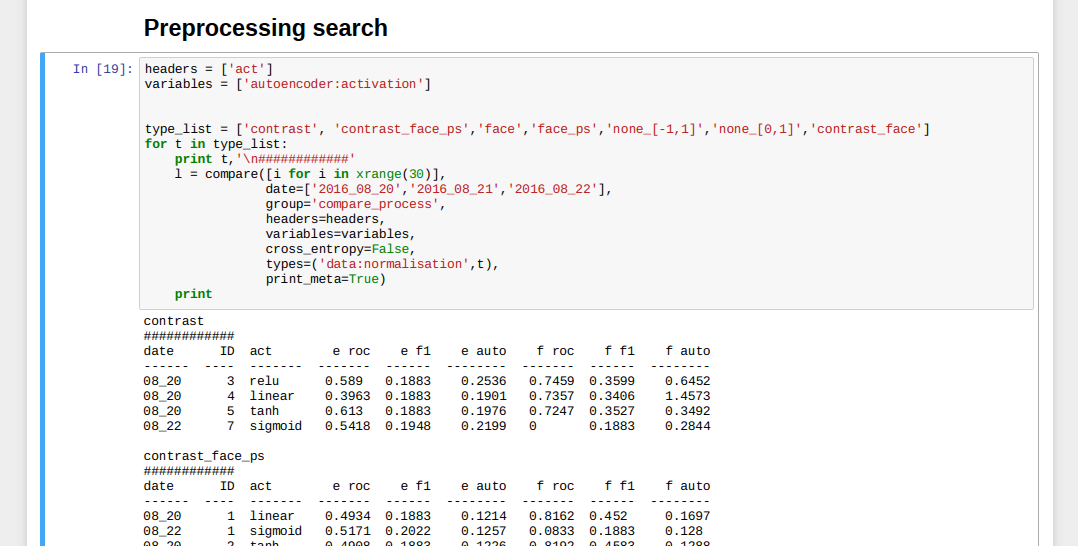
\includegraphics[width =0.8\hsize]{figures/notebook2.png}
                    \caption{{\bf compareResults.ipynb: }An example of an ipython script which compares the results of a selection of experiments,
                    this was used heavily to quickly produce the tables in the Results section.}
                    \label{fig:compareresults}
                    \end{figure}
                  \item {\bf viewResult.ipynb }
                  \begin{sloppypar} \textit{Visualises one run of main.py with many graphs and numerical results.}\end{sloppypar}
                    \begin{figure}[!h]
                    \centering
                    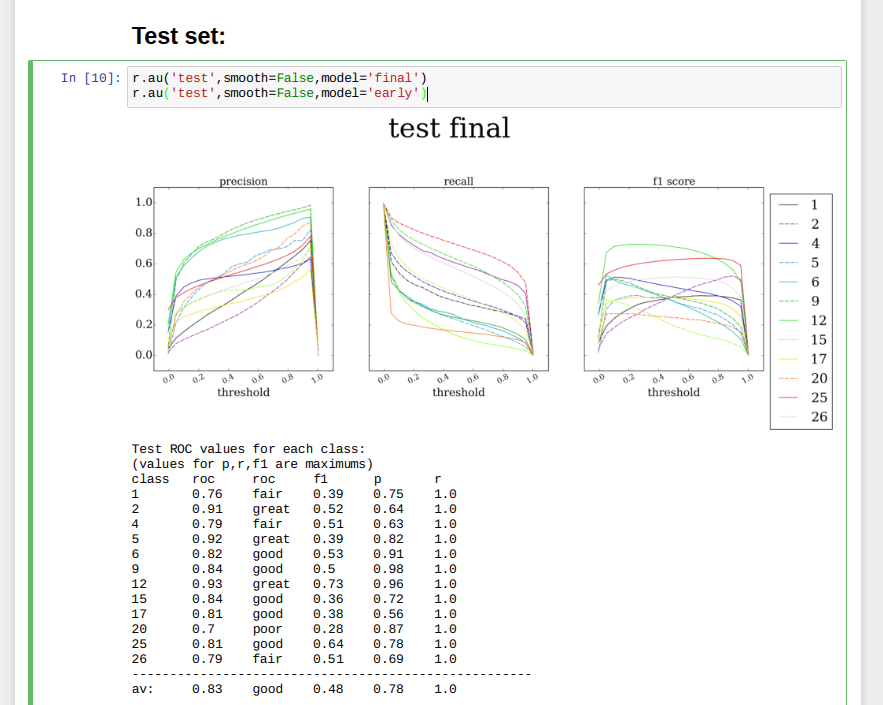
\includegraphics[width =0.8\hsize]{figures/notebook1.png}
                    \caption{{\bf viewResult.ipynb: } A small part of the notebook showing graphs related to F1, Precision and ROC for one experiment.}
                    \label{fig:viewresult}
                    \end{figure}
                  \item {\bf DisfaTest.ipynb }
                  \begin{sloppypar} \textit{Generates the graphs shown in section \ref{sec:methods}, this serves the purpose of
                    testing the preprocessing methods.}\end{sloppypar}
                \end{itemize}

      \end{itemize}
      }
